\chapter{Web 2.0}\label{ch:ch2}

\subsubsection{2.1.1}

According to a number of scholars, the rise of Twitter publishing had to lead a new level of informational openness in social networks and to increase of press freedom. At the same time, some recent studies have shown significant criticism towards political efficacy of Twitter [7] (нужен источник). We analyze Twitter as a part of the hybridized media system [6] (нужен источник) suggesting after Adam and Pfetsch [1] (нужен источник) that political dimension of hybridization and spill-over effects between different media will be specific to the socio-political context. In terms of the media system modernization [15] (нужен источник) and hybridization context, Russian media system is the one bearing both unique and post-Communist-specific features. In our research, we aim at analyzing the role of Twitter in the process of agenda setting in the hybridized media system in Russia and finding out if the use of Twitter potentially leads to the formation of the ‘crossroads of opinions' or, in contrast, to encapsulation of political discussion and further fragmentation of public discourse.Our research focuses on structural and content aspects of discussion on anti-migrant bashings in Biryulyovo (Moscow) in October 2013. Methods of research include automated web crawling, framing analysis via semantic coding, and interpretation of descriptive statistics. Preliminary results suggest unexpectedly high level of mediatization of the discussion. The ‘crossroads' nature of the discussion showed up but in such a way that makes Twitter differ from elite communicative milieus like the Russian Facebook.

\subsubsection{2.4.1}

The community-based structure of communication on social networking sites has long been a focus of scholarly attention. However, the problem of discovery and description of hidden communities, including defining the proper level of user aggregation, remains an important problem not yet resolved. Studies of online communities have clear social implications, as they allow for assessment of preference-based user grouping and the detection of socially hazardous groups. The aim of this study is to comparatively assess the algorithms that effectively analyze large user networks and extract hidden user communities from them. The results we have obtained show the most suitable algorithms for Twitter datasets of different volumes (dozen thousands, hundred thousands, and millions of tweets). We show that the Infomap and Leiden algorithms provide for the best results overall, and we advise testing a combination of these algorithms for detecting discursive communities based on user traits or views. We also show that the generalized K-means algorithm does not apply to big datasets, while a range of other algorithms tend to prioritize the detection of just one big community instead of many that would mirror the reality better. For isolating overlapping communities, the GANXiS algorithm should be used, while OSLOM is not advised. 

\subsubsection{2.4.2}

Despite disputable possibility of extension of analysis of social relations on Twitter to real life, Twitter discussions are still being under attention of scholars studying structures and meanings of news- and issue-based ad-hoc public discourse. One of the socially relevant aspects of Twitter studies is that of influencers -- accounts that produce impact, either inside or outside Twitter. But there is still no agreement in the research community on how to defme and measure who is an influencer: either by 'absolute figures' or by network analysis metrics; this issue is even rarely discussed. Politically, today's mediatized public sphere where traditional media play the role of information hubs is highly uneven in terms of access to opinion expression; it privileges institutional players, including political elites, corporations, and media themselves. Hopes that Twitter would provide a more equal space for public deliberation are still not proven enough. Using web crawling and manual assessment of Twitter ad-hoc discussion on the Biryulyovo bashings of 2013, we show that users who post or even get commented most do not make it to the positions of most 'central' users by network metrics. We also demonstrate that usen that rank high by betweenness and pagerank centntrality form circles of reciprocal commenting that show the social cleavage wider than the discussion itself.

\subsubsection{2.4.3}

Today, a range of research approaches is used to define the so-called influencers in discussions in social media, and one can trace both conceptual and methodological differences in how influencers are defined and tracked. We distinguish between ‘marketing’ and ‘deliberative’ conceptualization of influencers and between metrics based on absolute figures and those from social network analytics; combining them leads to better understanding of user activity and connectivity measures in defining influential users. We add to the existing research by asking whether user activity necessarily leads to better connectivity and by what metrics in online ad hoc discussions, and try to compare the structure of influencers. To do this, we use comparable outbursts of discussions on inter-ethnic conflicts related to immigration. We collect Twitter data on violent conflicts between host and re-settled groups in Russia and Germany and look at top20 user lists by eight parameters of activity and connectivity to assess the structure of influencers in terms of pro/contra-migrant cleavages and institutional belonging. Our results show that, in both discussions, the number of users involved matters most for becoming an influencer by betweenness and pagerank centralities. Also, contrary to expectations, Russian top users all in all are, in general, more neutral, while Germans are more divided, but in both countries pro-migrant media oppose anti-migrant informal leaders.

\subsubsection{2.4.4}

Abstractive summarization is a technique that allows for extracting condensed meanings from long texts, with a variety of potential practical applications. Nonetheless, today’s abstractive summarization research is limited to testing the models on various types of data, which brings only marginal improvements and does not lead to massive practical employment of the method. In particular, abstractive summarization is not used for social media research, where it would be very useful for opinion and topic mining due to the complications that social media data create for other methods of textual analysis. Of all social media, Reddit is most frequently used for testing new neural models of text summarization on large-scale datasets in English, without further testing on real-world smaller-size data in various languages or from various other platforms. Moreover, for social media, summarizing pools of texts (one-author posts, comment threads, discussion cascades, etc.) may bring crucial results relevant for social studies, which have not yet been tested. However, the existing methods of abstractive summarization are not fine-tuned for social media data and have next-to-never been applied to data from platforms beyond Reddit, nor for comments or non-English user texts. We address these research gaps by fine-tuning the newest Transformer-based neural network models LongFormer and T5 and testing them against BART, and on real-world data from Reddit, with improvements of up to 2\%. Then, we apply the best model (fine-tuned T5) to pools of comments from Reddit and assess the similarity of post and comment summarizations. Further, to overcome the 500-token limitation of T5 for analyzing social media pools that are usually bigger, we apply LongFormer Large and T5 Large to pools of tweets from a large-scale discussion on the Charlie Hebdo massacre in three languages and prove that pool summarizations may be used for detecting micro-shifts in agendas of networked discussions. Our results show, however, that additional learning is definitely needed for German and French, as the results for these languages are non-satisfactory, and more fine-tuning is needed even in English for Twitter data. Thus, we show that a ‘one-for-all’ neural-network summarization model is still impossible to reach, while fine-tuning for platform affordances works well. We also show that fine-tuned T5 works best for small-scale social media data, but LongFormer is helpful for larger-scale pool summarizations.

\subsubsection{2.4.5}

\textit{Objectives.} Social media have become a place where the bulk of grassroots political discussion takes place. Today, the growing body of research is dedicated to cumulative patterns on online deliberation, the predecessors of which were the concept of the spiral of silence, the silent majority hypothesis, and influencer studies. However, when applied to the dissonant, disruptive, and discontinued online discussions of today where gatewatching is much less predictable and cumulation of support is often accompanied by communicative aggression, these concepts need to be reconsidered and re-tested. Also, the current public communication online is much more multi-level than before; even within one platform, several communication layers may be defined, and their inter-relations in terms of public opinion aggregation remain under-studied. \textit{Research goal.} This paper aims at discovering patterns of cumulative deliberation in online communication. We first discuss the umbrella concept of cumulative deliberation. Then, we test the dynamics of the discussion on Belarusian oppositional YouTube in terms of impact of cross-account commenting on growth of commenting within the cross-account community and the overall discussion. \textit{Method and sampling.} We have collected the data by YouTube crawling. The data include all user comments of 2018 for six salient Belarusian oppositional accounts. To define the cross-account commenters, we used Gephi-based web graph reconstruction. We manually coded user posts for interactivity, aggression, and criticism. Dependencies in the dynamics of the discussion were tested by correlational and cluster analysis. \textit{Results.} We have discovered that users diverged into two mutually exclusive modes of expression, namely aggressive-dialogical and (self-)critical. Of the cross-account commenters, several users demonstrated ‘cumulative’ behavior and personal opinion bubbles. While there were nearly no dependencies discovered in the dynamics of user posting, criticism and self-criticism show capacity of spurring/diminishing the dynamics of public communication online, even if commenting on the whole is cumulative, not dialogical.

\subsubsection{2.4.6}

With the emergence of discussion platforms like Twitter, the hopes rose that computer-mediated public sphere would become more even in access to discussion than mass-mediatized public sphere of the late 20th century. Scholars have argued that it will eventually form an 'opinion crossroads' where conflicts would be discussed by all the parties involved. But today, existing research provides mixed evidence on whether ordinary users, rather than mainstream media and institutional actors, can become influencers in discussions on current issues, e.g. relations between host and migrant communities. We focus on the Twitter discussion about an inter-ethnic conflict in Moscow's Biryuliovo district in 2013 and aim at defining who were its real influencers by reconstructing the discussion's web graph, as well as analyzing and juxtaposing its metrics to figures indicating user activity. Our results show that, despite hyperactivity of media accounts, they were largely absent as deliberative influencers, but the place of influencers was occupied by politicized (nationalist and liberal) accounts, rather by eyewitness reporters or public figures.

\subsubsection{2.4.7}

With the emergence of discussion platforms like Twitter, the hopes rose that computermediated public sphere would become more even in access to discussion than massmediatized public sphere of the late 20th century. Scholars have argued that it will eventually form an ‘opinion crossroads’ where conflicts would be discussed by all the parties involved. But today, existing research provides mixed evidence on whether ordinary users, rather than mainstream media and institutional actors, can become influencers in discussions on current issues, e.g. relations between host and migrant communities. We focus on the Twitter discussion about an inter-ethnic conflict in Moscow’s Biryuliovo district in 2013, as well as the comparative ‘calm’ period in March 2014, and look at who were real influencers by reconstructing the discussion’s web graph, as well as analyzing and juxtaposing its metrics to figures indicating user activity. Our results show that ad hoc discussion differs dramatically from an issuebased one in terms of the influencer nature and composition; the role of active tweeting is questioned. We also show that nationalist accounts play a much bigger role than expected in both periods.

\subsubsection{2.5.1}

Конфликты с участием переселенцев «с глобального Юга» и их обсуждение в медиа и социальных сетях стали чертой современной публичной сферы в Европе и России. Сетевые дискуссии способны играть роль групп давления в формировании повестки обсуждения миграции и принятия политических решений, актуализируя как конфликтные, так и консенсусные общественные настроения. Важно знать, существуют ли закономерности в том, кого пользователи сети (в том числе иститутциональные) видят как виновников конфликтов и от кого ожидают его разрешения. Мы рассматриваем четыре конфликтные дискуссии в Твиттере в России и Германии 2013--2016 гг. и оцениваем связь статуса пользователя с паттернами присвоения вины и ответственности, а также сопоставляем дискурсивные стратегии обвинения в двух странах. Методология исследования включает веб-краулинг по заданному словарю, экспертную оценку аккаунтов пользователей, ручное кодирование твитов и описательную статистику. Итоги исследований говорят о том, что в целом обвинение направлено в первую очередь против трех групп: региональных властей, нацилнального лидера/правительства и иммигрантов; разрешения конфликтов пользователи ждут от федеральных властей, ответственных за изменение иммиграционной политики. Но если в Германии очевиден политический разлом между правыми (пронационалистическими) и левыми (феминистскими) стратегиями поиска виноватых, то в российском Твиттере доминирует обвинение и власти, и иммигрантов, а также распространены сниженные ожидания мирной политической разрядки межэтнической напряженности.

\subsubsection{2.5.2}

Recently, the growing role of social network users in content dissemination has brought to life the concept of secondary gatekeeping -- selection and republication of content already selected and published by traditional gatekeepers. Secondary gatekeeping is believed to be raising the media in-platform visibility, but it may also have negative effects such as adding to creation of echo chambers and deepening the gaps between conflicting views. Such studies are particularly relevant for emergencies or social conflicts where sharing relevant content may be crucial for lowering social unease. But till today the nature of secondary gatekeeping remains highly understudied. We have conducted a comparative study of three \textit{ad-hoc} Twitter discussions on heated ethnic/racial conflicts in the USA (Ferguson riots), Germany (Köln mass abuse), and Russia (Biryulyovo anti-migrant bashings) to assess the patterns of content sharing by active discussants. We used vocabulary-based web crawling and human coding of over 1,000 tweets in randomized samples. Our results show that, in all cases, there’s weak but significant correlation between the type of user and his/her attitude to minority with the attitudes expressed in content, while it is not always true that users prefer the same gatekeeper type, e.g. online or social media. As difference between individual users remains statistically significant, this may mean that the nature of heated \textit{ad-hoc} discussions facilitates formation of ‘individual-level filter bubbles’ in addition to bigger echo chambers.

\subsubsection{2.5.3}

With growth of Internet communication, hopes rose that online discussions will equalize ordinary users and institutional discussants. But what roles traditional media play in online discussions remains under-researched. We argue that mediatization of Twitter discourse is worth studying, as activity of registered media in online discussions may play a role in preserving the “offline” deliberative inequalities. To assess the roles of media in Twitter discussions, we look at two structural aspects of their presence: posting activity and users’ sharing of media content -- within heated \textit{ad hoc} Twitter discussions on inter-ethnic conflicts in Russia, the USA, and Germany. Our findings show huge national differences in mediatization patterns, including the roles of political media. But also we see that, in all the three cases, the discourse is shaped by “white majority media”, and outlets that would represent the oppressed minority are virtually absent in both posting and link sharing patterns.

\subsubsection{2.5.4}

Online communication platforms have rapidly become a substantial element of e-governance processes in Europe and beyond. Today, research has shown that, in cases of social unrest and/or emergency, political actors responsible for their resolution are able to efficiently use microblogging platforms (including Twitter) to promote the discourse of harmonization. But in today's Russia, where the growth of inter-ethnic conflicts between the re-settlers from the post-Soviet South (Central Asia and South Caucasus) and the host communities in cities and towns has coincided with the growth of online communication milieus and their radicalization, political actors as well as NGOs seem to play minor roles in online communication management, including the cases of social unrest. We explore two Twitter discussions on inter-ethnic conflicts in Moscow to describe the presence of political actors, their roles in conflict resolution, and the patterns of expectations of other users towards the politicians. We discover extremely low political participation, as well as the phenomenon of 'radical replacement' of the roles of political emergency managers by nationalist users.

\subsubsection{2.5.5}

Embeddedness of politicians and political organizations in a discussion defines its level of institutionalization and creates a public arena for collaboration between publics and institutional actors. Thus, testing whether traditional hierarchies (in terms of presence of politically institutionalized actors) show up in online discussions deserves scholarly research. Moreover, it is also important to see whether more democratic societies show patterns of public involvement of politically institutionalized users that would differ from those in more authoritarian contexts.

To assess the ‘influencer’ status of politically institutionalized actors on Twitter cross-culturally, we have selected conflictual Twitter discussions in Germany, the USA, and Russia, all based on violent inter-ethnic clashes. Using vocabulary-based web crawling, we collected data on them and formed samples of top users selected by four activity metrics and five network metrics, to assess the positions of political users in the top lists and correlations of user status with their top list ranks. To this, we added qualitative assessment of presence of political users in comparative perspective.

Our results show that, in all the cases, presence of political actors in online discussions is scarce; also, political actors tend to fail to link user groups or stay in the center of discussion. There is also meaningful divergence of Russia from the pattern that Germany and the USA show: while in these countries politicians gain user attention based on content, in Russia it is the status itself that matters, and political users tend to gain weight in the discussion structure despite low attention levels.

\subsubsection{2.5.6}

YouTube-based discussions are a growing area of academic attention. However, we still lack knowledge on whether YouTube provides for forming critical publics in countries with no established democratic tradition. To address this question, we study commenting to Belarusian oppositional YouTube blogs in advance of the major wave of Belarusian post-election protests of 2020. Based on the crawled data of the whole year of 2018 for six Belarusian political videoblogs, we define the structure of the commenters’ community, detect the core commenters, and assess their discourse for aggression, orientation of dialogue, direction of criticism, and antagonism/agonism. We show that, on Belarusian YouTube, the commenters represented a genuine adversarial self-critical public with cumulative patterns of solidarity formation and find markers of readiness for the protest spillover.

\section{Концептуальное назначение}\label{sec:ch2/sec1}

%\begin{figure}[ht]
%    \centerfloat{
%        \includegraphics[scale=0.27]{latex}
%    }
%    \caption{TeX.}\label{fig:latex}
%\end{figure}
%
%Для выравнивания изображения по-центру используется команда \verb+\centerfloat+, которая является во
%многом улучшенной версией встроенной команды \verb+\centering+.

\section{Принципы построения ресурсов}\label{sec:ch2/sect2}

%А это две картинки под общим номером и названием:
%\begin{figure}[ht]
%    \begin{minipage}[b][][b]{0.49\linewidth}\centering
%        \includegraphics[width=0.5\linewidth]{knuth1} \\ а)
%    \end{minipage}
%    \hfill
%    \begin{minipage}[b][][b]{0.49\linewidth}\centering
%        \includegraphics[width=0.5\linewidth]{knuth2} \\ б)
%    \end{minipage}
%    \caption{Очень длинная подпись к изображению,
%        на котором представлены две фотографии Дональда Кнута}
%    \label{fig:knuth}
%\end{figure}
%
%Те~же~две картинки под~общим номером и~названием,
%но с автоматизированной нумерацией подрисунков:
%\begin{figure}[ht]
%    \centerfloat{
%        \hfill
%        \subcaptionbox[List-of-Figures entry]{Первый подрисунок\label{fig:knuth_2-1}}{%
%            \includegraphics[width=0.25\linewidth]{knuth1}}
%        \hfill
%        \subcaptionbox{\label{fig:knuth_2-2}}{%
%            \includegraphics[width=0.25\linewidth]{knuth2}}
%        \hfill
%        \subcaptionbox{Третий подрисунок, подпись к которому
%            не~помещается на~одной строке}{%
%            \includegraphics[width=0.3\linewidth]{example-image-c}}
%        \hfill
%    }
%    \legend{Подрисуночный текст, описывающий обозначения, например. Согласно
%        ГОСТ 2.105, пункт 4.3.1, располагается перед наименованием рисунка.}
%    \caption[Этот текст попадает в названия рисунков в списке рисунков]{Очень
%        длинная подпись к второму изображению, на~котором представлены две
%        фотографии Дональда Кнута}\label{fig:knuth_2}
%\end{figure}
%
%На рисунке~\cref{fig:knuth_2-1} показан Дональд Кнут без головного убора.
%На рисунке~\cref{fig:knuth_2}\subcaptionref*{fig:knuth_2-2}
%показан Дональд Кнут в головном уборе.
%
%Возможно вставлять векторные картинки, рассчитываемые \LaTeX\ <<на~лету>>
%с~их~предварительной компиляцией. Надписи в таких рисунках будут выполнены
%тем же~шрифтом, который указан для документа в целом.
%На~рисунке~\cref{fig:tikz_example} на~странице~\pageref{fig:tikz_example}
%представлен пример схемы, рассчитываемой пакетом \verb|tikz| <<на~лету>>.
%Для ускорения компиляции, подобные рисунки могут быть <<кешированы>>, что
%определяется настройками в~\verb|common/setup.tex|.
%Причём имя предкомпилированного
%файла и~папка расположения таких файлов могут быть отдельно заданы,
%что удобно, если не~для подготовки диссертации,
%то~для подготовки научных публикаций.
%\begin{figure}[ht]
%    \centerfloat{
%        \ifdefmacro{\tikzsetnextfilename}{\tikzsetnextfilename{tikz_example_compiled}}{}% присваиваемое предкомпилированному pdf имя файла (не обязательно)
%        %\input{Dissertation/images/tikz_scheme.tikz}
%
%    }
%    \legend{}
%    \caption[Пример \texttt{tikz} схемы]{Пример рисунка, рассчитываемого
%        \texttt{tikz}, который может быть предкомпилирован}\label{fig:tikz_example}
%\end{figure}
%
%Множество программ имеют либо встроенную возможность экспортировать векторную
%графику кодом \verb|tikz|, либо соответствующий пакет расширения.
%Например, в GeoGebra есть встроенный экспорт,
%для Inkscape есть пакет svg2tikz,
%для Python есть пакет tikzplotlib,
%для R есть пакет tikzdevice.

\section{Сбор данных}\label{sec:ch2/sec3}

%\noindent Нумерованный список:
%\begin{enumerate}
%    \item Первый пункт.
%    \item Второй пункт.
%    \item Третий пункт.
%\end{enumerate}
%
%\noindent Маркированный список:
%\begin{itemize}
%    \item Первый пункт.
%    \item Второй пункт.
%    \item Третий пункт.
%\end{itemize}
%
%\noindent Вложенные списки:
%\begin{itemize}
%    \item Имеется маркированный список.
%          \begin{enumerate}
%              \item В нём лежит нумерованный список,
%              \item в котором
%                    \begin{itemize}
%                        \item лежит ещё один маркированный список.
%                    \end{itemize}
%          \end{enumerate}
%\end{itemize}
%
%\noindent Нумерованные вложенные списки:
%\begin{enumerate}
%    \item Первый пункт.
%    \item Второй пункт.
%    \item Вообще, по ГОСТ 2.105 первый уровень нумерации
%          (при необходимости ссылки в тексте документа на одно из перечислений)
%          идёт буквами русского или латинского алфавитов,
%          а второй "--- цифрами со~скобками.
%          Здесь отходим от ГОСТ.
%          \begin{enumerate}
%              \item в нём лежит нумерованный список,
%              \item в котором
%                    \begin{enumerate}
%                        \item ещё один нумерованный список,
%                        \item третий уровень нумерации не нормирован ГОСТ 2.105;
%                        \item обращаем внимание на строчность букв,
%                        \item в этом списке
%                              \begin{itemize}
%                                  \item лежит ещё один маркированный список.
%                              \end{itemize}
%                    \end{enumerate}
%
%          \end{enumerate}
%
%    \item Четвёртый пункт.
%\end{enumerate}

\section{Анализ пользовательских Web-графов}\label{sec:ch2/sec4}

\subsection{Comparing influencers: activity vs. connectivity measures in defining key actors in twitter \textit{ad hoc} discussions on migrants in Germany and Russia}\label{subsec:ch2/sec4/sub3}

\subsubsection{1. Introduction}

Uneven representation of group interest in mediatized public discussions has been established in the research literature \cite{Nieminen} as one of the fundamental problems of public communication and public decision-making. Among the reasons for that, there is representation of newsmakers privileging institutional actors vs. ordinary citizens as \textit{vox populi} \cite{ScheufeleTewksbury}. Since Internet had emerged as a public communicative space less dependent on media, scholars expressed hopes that networked communication would provide for equalizing citizens with institutional actors within public discussions \cite{White1997} bypassing media who used to serve as gatekeepers of public agendas \cite{White1950}. But, till today, horizontalization of discursive relations online remains highly disputable \cite{Fuchs}; moreover, new societal cleavages emerge in hybrid media systems \cite{Chadwick} due to digital divide, interest- and value-based variance in media diets, and growing platform- oriented fragmentation of public arenas.

In online communicative milieus, the figures of \textit{newsmaker}, \textit{informer}, and \textit{opinion leader} are re-conceptualized as that of \textit{influencer} \cite{PattersonGrennyMaxfield}, partly based on an older idea of ‘influential’ \cite{Rogers}. Influencers combine beyond-the-average capacities of information dissemination with those of casting impact upon users’ opinions and formation of discussion circles often described as echo chambers \cite{Wallsten}, and thus are key structural elements of networked discussions \cite{Castells2007,BakshyRosennMarlow}.

Despite influencers’ expected crucial role in reshaping power relations between institutional and non-institutional participants of online discussions, they are, till today, under-studied in such aspects as dependence of influencer position upon user activity, institutional status, or taking sides in conflict. Social network analysis (SNA) tries to predict influencers technically, based on their activity and metadata, as well as on the discussion graph structure; other important works explore the interplay between the nature of the publics and constellations of influencers \cite{Habermas,Dahlgren,BrunsBurgess,Papacharissi,BrunsHighfeld2016}. Within this research cluster, Twitter as a microblogging platform has gained particular attention, but it is yet unclear whether this platform tends to democratize influencers in the so-called \textit{ad hoc} public discussions that rapidly rise and disseminate on events of high social relevance or on issues with high potential of social polarization.

To a large extent, this is due to the fact that very different approaches to defining and detecting influencers co-exist in computer science and communication disciplines. Earlier, we traced at least two concepts of influencer (based on user activity and user connectivity, respectively), as well as a methodological divide in detecting influencers via absolute-figure metrics and SNA metrics \cite{BodrunovaLitvinenkoBlekanov2016}; we also stated that few attempts had been made to juxtapose these ways of detecting influencers. Also, comparative studies beyond the Western and Arab Spring countries remain rare \cite{HladikStetka}.

Thus, the aim of this paper is twofold. First, we assess whether user activity necessarily leads to better connectivity, and by what metrics. Then, we try to compare the structure of influencers across countries in terms of their institutional belonging and pro-/anti-migrant stance. We do this by collecting and analyzing data on the Twitter discussion around anti-migrant bashings in Biryuliovo (Moscow) in 2013 and the one around the mass harassment in Cologne in 2016. To accomplish this, we have collected the discussion content, selected the metrics, applied them and formed user lists by activity and connectivity metrics (betweenness and pagerank centralities). We manually assessed the listed accounts to position them institutionally and politically.

Section 2 presents our conceptualization of ‘marketing’ vs. ‘deliberative’ influen- cers, while Sect. 3 reviews today’s approaches to defining influencers, including those based on user activity and connectivity metrics. Section 4 describes the cases, research hypotheses, and our methodology. Section 5 discusses our results.

\subsubsection{2. Actor Disparities in \textit{Ad Hoc} Twitter Discussions}

By 1990s, the public sphere theory had already stated that public discussions were arenas of high disparities in terms of who formed the opinions and influenced the discussion agendas. As mentioned above, institutional and elite representatives were naturally preferred by media; moreover, media themselves became the key nodes in information networks and performed agenda setting \cite{McCombsShaw,McCombs}. Another reason for criticism of media-based public spheres was their oppressive majority-oriented discourse \cite{Fraser,LaclauMouffe,FentonDowney,Dahlberg}; a lot of efforts have been put by countries in Europe and beyond to establish public media that would encompass at least some minority views.

With the rise of online platforms, hopes for better access of citizens to public discussion first rose \cite{Fuchs} and then faded, as both social \cite{Nakamura} and communicative \cite{Daniels} offline divides were accompanied by new disparities emerging due to divergent media consumption \cite{PfetschAdam,BodrunovaLitvinenko} and digital divide \cite{Norris,VanDeursenVanDijk}, among other reasons. Not even asking whether Twitter discussions have any impact upon real-world policymaking, scholars doubt even whether ‘Habermas is on Twitter’ \cite{BrunsHighfeld2016} \cite[p.~31]{Murthy}. Out of this, a range of research agendas have emerged on who become discussion leaders (influencers) and whether the disparities in influence persist. Also, we need to know how we define and detect the influencers, as their detection appears to be measure-dependent.

\textit{Defining an Influencer.} SNA is widely used to show deviant users in Twitter discussions. As we stated before \cite{BodrunovaLitvinenkoBlekanov2016}, there are at least three major divisions in SNA-based influencer studies that define influencers in differing ways.

Here, we will only shortly reconstruct our logic and show applicability of this logic to comparative studies. Thus, the three divisions may be conceptualized as follows. The first one is between ‘marketing’ and ‘deliberative’ influencers. The former generates a self-oriented ‘long tail’ of attention and support \cite[p.~1261]{DuboisGaffney} \cite{Aquino}; here, key characteristics of an influencer are \(N_{followers}\), the quantity and regularity of posting, and the vastness of ‘support waves’ of liking and retweeting. The latter, ‘deliberative’ influ- encer, helps in formation of a politically relevant and effective discussion by linking user groups with varying or even opposing views, as well as of intertwining topic-based echo chambers; also, such a user is linked to the maximum number of other users within the discussion by interacting with them. As inclusiveness and horizontality \cite{Papacharissi2010}, along with rationality and orientation to consensus, are key features of an effective ‘field of discursive connections’ \cite[p.~37]{Calhoun}, deliberative influencers are key for formation of ‘opinion crossroads’ \cite{BodrunovaLitvinenko,VanDeursenVanDijk} as a metaphor of an all-involving public discussion. Structurally, inter-linkage between clusters in a discussion and \(N_{users}\) involved in commenting and retweeting becomes the feature that defines an influencer. We consider these approaches mutually amplifying, as they both, in a way, are extensions of theory of two-step communication flow via opinion leaders \cite{Katz}.

To add, two more divisions may be traced: first, the one between user activity metrics (\(N_{posts}\), \(N_{likes}\), \(N_{retweets}\), \(N_{comments}\) left, \(N_{users}\) followed, \(N_{users}\) involved by a given user into any type of interaction) and user connectivity metrics (\(N_{likes}\), \(N_{retweets}\), \(N_{comments}\) received, \(N_{followers}\), \(N_{users}\) interacting with a given user, and centrality metrics that describe a user’s position in the web graph). And second, the same metrics are divided into absolute-figure ones measured for every user independently and graph-based metrics that, for every user, depend on the overall graph configuration \cite{BodrunovaLitvinenkoBlekanov2016}.

\textit{Conceptual Limitations in Twitter Studies of Influencers.} But before discussing particular ways of detecting influencers on Twitter, we need to mention that there are limitations for that; they are linked to the nature of the discussion, its level of rationality, and inherent Twitter mechanisms that technically privilege certain actors \cite{BodrunovaLitvinenkoBlekanov2016}.

In short, the first limitation is linked to the fact that ‘issue publics’ \cite[p.~422]{Habermas} \cite[p.~108]{VanDeursenVanDijk}, or \textit{ad hoc} publics \cite{BrunsBurgess}, become affective \cite{Papacharissi} and quickly rise and dissolve \cite[p.~74]{Dahlgren}. This, in its turn, raises two issues: (1) that of representability of \textit{ad hoc} discussion for stable discursive patterns outside the time of the event; (2) comparability of \textit{ad hoc} discussions in terms of their structure and the conclusions they allow for. In response to this, we may state that our experiments (work in progress) show that the structure of \textit{ad hoc} discussions changes the same way in six different discussions if isolated users are eliminated; that is, the patterns of \textit{ad hoc} discussions are, at least partly, comparable. In future, we will also test their comparability with stable discussions.

The issue of rationality has been debated among scholars since the appearance of Twitter itself. Twitter pessimists claim that the platform is home for depoliticized trivial content full of ‘white noise’ \cite{HartleyGreen} and subjected to slacktivist practices \cite{Morozov}. Other studies, though, show that migroblogging changes news agendas \cite{BroersmaGraham}, generates ‘sub-political’ discussion topics \cite{LindgrenLundstrom}, and may result into ‘self-generated public opinion’, as in long-text blogs \cite{KoltsovaKoltcov}; we share the latter opinion. Also, scholars have called Twitter the quickest platform for expression of public sentiment \cite{BrunsBurgessCrawford}; this is why we cannot dismiss the Twitter influencers’ potential of shaping the discussions.

The third limitation poses the question of structural limitations for all-involving discussion. Twitter networks resemble information-sharing ones and not offline social networks \cite[p.~264]{BastosRaimundoTravitzki} and, thus, privilege ‘gatewatchers’ \cite{Bruns} or ‘gateways’ \cite{BastosRaimundoTravitzki} who multiply and disseminate information from both outside the network and from influ- encers, as Twitter networks demonstrate ‘highly skewed distribution of followers and a low rate of reciprocated ties’ \cite[p.~263]{BastosRaimundoTravitzki}. But in our paper we try to see whether active users with a particular position towards migrants get to the influencer lists; later, we may check whether the structure of the network played a role in their promotion.

\subsubsection{3. Absolute Figures vs. Centrality Metrics in Detecting Influencers}

In our earlier case study, we have showed that existing research actually rarely links absolute-figure metrics to SNA-based graph-dependent metrics (centralities) \cite{BodrunovaBlekanovMaksimov}. Extremely wide SNA literature is dedicated to predicting the key nodes in discussion networks; a smaller bunch of works applies the network-based metrics to Twitter discussions (as examples, see \cite{DuboisGaffney,AlmindIngwersen}), using not only single metrics but also their combinations \cite{KwakLeePark,GonzalezBailonBorgeHolthoeferMoreno} and case-specific derivatives \cite{MairederWeeksDeZuniga}.

Several of these works have focused on the institutional nature of the key network nodes; mainly, researchers are looking at whether media continue to be information flow hubs -- and express significant doubts. Thus, authors \cite{BastosRaimundoTravitzki} have shown that it was content that mattered for generating ‘highly replicated messages... without relying on the activity of user hubs’ \cite[p.~260]{BastosRaimundoTravitzki}, and that the role of media outlets in forming retweet waves was much exaggerated \cite[p.~269]{AlmindIngwersen}. Other authors \cite{DuboisGaffney} have shown that media remained influencers only by indegree and eigenvalue metrics; another research group \cite{HilbertVasquezHalpern} has demonstrated that new groups of influential users join experts and media. Thus, we expect that media would still be among network-detected influencers but they will not be the leading ones.

But at the same time, research that uses absolute-figure metrics provides a more nuanced picture on who is labeled as influencer, which metrics to use for detecting them, and whether institutional (political, media, economic etc.) users remain among them. Earlier, we have shown that the majority of researchers have named \(N_{retweets}\) the most efficient metric to detect an influencer \cite{BodrunovaLitvinenkoBlekanov2016}. But other authors warn that \(N_{retweets}\) cannot actually help differentiate between ‘having a following’ due, e.g., a big number of tweets by a given user or a celebrity -- and ‘being seen as an expert’ whose tweets are genuinely shared more than those of other users \cite[p.~1263]{DuboisGaffney}; \(N_{tweets}\) has been shown to be a mediating factor for other metrics \cite{Jungherr}. This understanding corresponds to our ‘marketing’ vs. ‘deliberative influencers’ division.

Also, most of these works insist that institutionalized users remain highly influential in how discussions develop. Of course this partly due to another view on influencer as on ‘prestigious actor whose position is approved by the audience and who initiates more support than criticism’ \cite{Adam}, which does not take into account the user’s position in the network. In this line of research, several case studies have proved that Twitter strengthens the pre-existing hierarchies with media and political leaders \cite{WuHofmanMason,VaccariValerianiBarbera,JungherrJuergens}, as well as experts and long-established institutions \cite{FoxZickuhrSmith,Page}, still playing the key role in information dissemination. Using a composite measure named ‘mentions’ (that comprises several absolute-figure metrics), author \cite{Vis} shows that journalists and mainstream media were dominating the top100 accounts in the Twitter coverage of the UK 2011 riots. Similar results were received for New Zealand \cite{Bruns2014} where, of top16 Twitter accounts by retweet \& comment, 11 were institutional and included media. This may happen because journalists often retweet other journalists \cite{LotanGraeffAnanny}, but this can hardly influence the top lists selected out of several hundred thousand users
.
So far, only rare works tried to combine or juxtapose the absolute and network-based metrics \cite{BodrunovaLitvinenkoBlekanov2016,Adam,GruzdRoy,XuSangBlasiola}. To see the correlations between the two types of metrics, we will use the scheme we had elaborated earlier \cite{BodrunovaLitvinenkoBlekanov2016}. We will use both activity/connectivity and absolute/network-based divisions to describe the metrics we will juxtapose. Thus, the metrics we will use for top list formation are the following:

\begin{itemize}
	\item activity, absolute: \(N_{tweets}\);
	\item activity, network-based: outdegree centrality;
	\item connectivity, absolute: \(N_{retweets}\), \(N_{comments}\), \(N_{recom}\) -- retweets and comments combined (as it was conceptualized in \cite{Bruns2014});
	\item connectivity, network-based: indegree, betweenness, and pagerank centralities.
\end{itemize}

\subsubsection{4. The Cases, Research Hypotheses, and Methodology of the Study}

To formulate our research questions more precisely, we also need to take into con- sideration the context of the cases under scrutiny. The relevant aspects include the expectations from the Russian and German Twittersphere formulated in the existing research; the description of the cases; the societal cleavages inside it. This is done to help form our expectations of who would be the influencers within the discussions.

\paragraph{4.1 The Inter-ethnic Conflicts in Germany and Russia and Their Social and Communicative Context} 

To explore the issues described above, we have focused on comparable conflictual \textit{ad hoc} discussions. The topic of migrant crime and the following anti-migrant uprising provides cases that possess the following features: they have a rapid violent trigger, cause social polarization and street action, involve authorities, and get to national Twitter trending topics.

\textit{The German case.} According to statista.com, the number of regular Twitter users in Germany in 2015 was only 1.73 million (2\% of the population), with about twice that number using it occasionally \cite{Kissane}, and it seems not to grow since 2010 \cite{TumasjanSprengerSadner}.

The German media system belongs to the democratic corporatist model \cite{HallinMancini} with a strong tradition of freedom of expression combined with the tradition of corporatism, including the leading role of public TV. Also, the press market, despite the adherence to the notion of objectivity, is characterized by a degree of political polarization and media-political parallelism, as well as by powerful tabloids. The German Twitter, though being an undeniable news alert arena and one of the political facilitation tools in mass actions, has generated virtually no research on its structure and discussion features. Thus, our expectations are based on the overall structure of the media market, traditions of balanced reporting and public deliberation, and specific features of the German media market and civil society stated above. Thus, we expect German state actors and NGOs to be present in the discussion and perhaps even to become the discussion centers; supra-national mainstream media (like foreign newspapers or Euronews TV channel) will also be present.

The event under our scrutiny is the Köln mass harassment. During the New Year’s Eve 2015/2016 in Köln (Cologne), numerous sexual assaults were committed on women by groups of young men, allegedly mainly from the North African and Arab countries. The attacks triggered a new wave of far-right protests of the ultraconservative party ‘Alternative für Deutschland’ (AfD) and anti-migrants movement ‘Pegida’. Public support for refugee-welcoming politics of Angela Merkel has significantly dropped within several weeks \cite{Dearden}. The national media reported about the attacks with delay of several days, which led to new accusations of the mainstream media in pro-migrant bias and to escalation of the debate about the ‘lying press’ (‘Lügenpresse’) by AfD and Pegida. The Parliamentary Assembly of the Council of Europe reacted with a debate under urgent procedure on January 25, 2016, stating in Resolution 13961 that ‘media hold an important responsibility to report on objective facts without stigmatization. Partial, late or dishonest media reporting on crimes can feed in con- spiracy theories and fuel hatred against a part of the population. It can also contribute to mistrust in the authorities and the media’.

The Russian Case. After 1991, the Russian media system has seen fundamental transformation but, in political respect, it remained mostly post-Soviet \cite{Vartanova}. Today, the country’s media sphere is highly fractured along the lines of value-based cleavages between small cosmopolitan hyper-urban and huge mid-urban post-Soviet population clusters \cite{BodrunovaLitvinenko2013,BodrunovaLitvinenkoGavraYakunin}. Online, this division shows up in formation of platform-wide political echo chambers \cite{BodrunovaLitvinenkoGavraYakunin}, with the Russian Facebook serving as the best example.

Research on Russian Twitter is as well extremely scarce; it is hard even to estimate the overall use of Twitter in Russia. As for August 2015, figures varied from 8 to 11 mln subscribers, of which around 50\% seemed to be active users (used Twitter once a month or more, as estimated by TASS). The existing research on Russian Twitter provides mixed evidence on whether Twitter in Russia can play a role of an ‘opinion crossroads’. Several works have proved that political representation of pro- and anti-‘systemic’ actors on the Russian Twitter is virtually equal \cite{Greene,NikiporetsTakigawa}, but at the same time others stated that topic-based clusters with clear political bias were evident in earlier years \cite{BarashKelly}. Importantly, the latter work also stated the absence of any distinct nationalist clusters in the Russian blogs and on Twitter in particular. Except for our earlier works \cite{BodrunovaLitvinenkoBlekanov2016,BodrunovaBlekanovMaksimov}, there was no substantial attempt to study the nature and structural roles of influencers on the Russian Twitter. The newest work \cite{SanovichStukalPenfoldBrown} also proved extremely high ‘botization’ of political topics on the Russian Twitter; this is why we take as case the discussion of almost 4 years ago when it was not yet the case.

The events we analyze -- anti-migrant bashings in Biryuliovo district of Moscow -- happened in October 2013 and were in Twitter Trending Topics for over two days. The timeline included akilling of a Muscovite Egor Scherbakov by an Uzbek named Orkhan Zeinalov, the bashings at Biryuza trade center, its warehouse and the surroundings in Biryuliovo where the alleged killer should have resided along with many of his fellows, and the subsequent police street actions, several ‘gatherings’ of the locals, and arrest and trial of the suspect; the events were also accompanied by statements of federal and Moscow authorities. Thus, the actors that we may trace were: authorities (federal, Moscow, local); police; eyewitnesses; migrants. As the case was reported in federal and local media, we also expect high level of media involvement.

Expectations in Terms of Influencer Structure and Positioning. In both countries, we expect institutional actors to dominate top user lists, despite high levels of eyewitness posting. We expect national and local authorities, media, and police to be the main influencers; to a smaller extent, we expect NGOs and other pro-migrant speakers to form the lists. According to earlier research, we expect neither nationalists nor migrants to be highly influential in the Russian case, while we may expect anti-migrant citizens to show up in both cases; but taking into consideration the traditions of public discussion in Germany, we expect users and media to be mostly neutral.

\paragraph{4.2 Research Questions} 

Based on everything aforementioned, we have formulated four research questions.

\paragraph{RQ1. Do the users that post most become discussion centers in both absolute and network-based metrics? That is, does \(N_{tweets}\) significantly correlates to \(N_{retweets}\), \(N_{comments}\), \(N_{recom}\), outdegree, betweenness, and pagerank centralities in both cases?}

\paragraph{RQ2. Do institutionalized users dominate over ordinary users by both activity and connectivity metrics? Do the patterns of institutionalization differ a lot? We expect that, for Russia, pro- and anti-migrant users (like NGOs and nationalists) will be absent from both the lists of active (\(N_{tweets}\), indegree) and ‘central’ (betweenness and pagerank) top user lists; but in Germany we expect more political actors, social organizations, and NGOs to form the lists.}

\paragraph{RQ3. Do media occupy significant place in top user lists? Within the lists, are media of all views are represented?}

\paragraph{RQ4. Are institutional and most non-institutional top users neutral in terms of taking sides in the conflict?}

\paragraph{4.3 Methodology and Research Process} 

To collect the discussion bulk, we conducted vocabulary-based web crawling; then, we reconstructed the discussion web graphs. For this, we developed a specialized web crawler \cite{BlekanovSergeevMartynenko}. We used our own software to overcome limitations common for openly available API-based analogs; our algorithm is human-like, which allowed for unfolding of the discussion in the past and trespassing the time and quantity upload limits. To form the vocabularies, we first collected relevant keywords and hashtags at trendinalia.com and double-checked the lists on two other Twitter trending topics trackers.

Then, we added more hashtags based on manual snowballing of tweets in over 1,000 tweets for both cases. The vocabularies for Russia included 6 main hashtags/keywords, and for Germany -- 15 hashtags/keywords.

For Russia, the research period chosen was October 1 to 31, 2013, to capture the outburst of the discussion and its long tail. 3,574 users with 10,715 posts were identified as a result of crawling and formed the core dataset. One step further in crawling was made to identify those who commented or retweeted the collected tweets, to calculate properly the number of comments and retweets; this returned 12,040 users. For Germany, a similar strategy of uploading (January 1 to 31, 2016) discovered a significantly bigger discussion of 12,382 users involved with 64,874 posts posted; one step further returned 40,117 users.

For comparison, we used the user lists from the core datasets, but the data on commenting and retweeting for individual users are taken from the bigger datasets.

Then, we have conducted the following procedures:
\begin{enumerate}
	\item To calculate the SNA metrics, we reconstructed the discussion graphs. The graphs themselves were non-directed (as we were not interested in directions of interactions, only in numbers), but our data allowed for calculating in-/outdegrees independently.
	
	\item From the graphs, we received the values for the chosen variables: \(N_{tweets}\), \(N_{retweets}\), \(N_{comments}\), \(N_{recom}\), indegree, outdegree, betweenness, and pagerank for the core datasets.
	
	\item After that, we formed additional dataset of users with \(N_{tweets} \geq 10\) to include only those who actively participated in the discussion. This was done in order to exclude the discussion ‘long tails’ with large number of users who, though, posted only a few tweets each and, thus, would distort the results true for active users. For Germany, the list included 1,211 users; for Russia, only 178 users.
	
	\item Then, we conducted descriptive statistics (Spearman rho) to see to what extent the chosen metrics correlate in the core datasets and the datasets with \(N_{tweets} \ge 10\) (see Tables~\cref{tab:spearmanCorrelationRussiaCore} and~\cref{tab:spearmanCorrelationRussiaActive} for Russia and Tables~\cref{tab:spearmanCorrelationGermanyCore} and~\cref{tab:spearmanCorrelationGermanyActive} for Germany). We considered the use of Spearman’s rho appropriate despite we realized that absolute figures, including \(N_{tweets}\) and in-/outdegree values may play a role in formation of other centrality metrics, and we expect them to correlate, but it is the strength of correlation that we will be looking at. Also, as stated above, betweenness and pagerank are network-dependent, while in-/outdegree are calculated as absolute numbers of user interactions.
	
	\item We manually checked the user top lists, to assess the patterns user transposition from the lists by activity metrics to the lists by connectivity metrics, and those by absolute figures -- to those by network metrics; we also marked their institutional belonging and pro-/anti-migrant position (see Figs.~\cref{fig:topUsersRussia} and~\cref{fig:topUsersGermany}). To do so, we checked a user’s self-description, the collected tweets, and the user’s tweets closer to nowadays.
\end{enumerate}

The results assessed in comparative perspective are presented below.

\begin{table}[ht]%
	\centering
	\caption{Spearman’s correlation between activity and connectivity measures in Russia for the core dataset \((N_{users} = 3,574)\).}%
	\label{tab:spearmanCorrelationRussiaCore}% label всегда желательно идти после caption
	\begin{adjustbox}{width=1\textwidth}
		\small
		\begin{tabular}{ c  c  c  c  c  c  c  c  c }% Вертикальные полосы не используются принципиально, как и лишние горизонтальные (допускается по ГОСТ 2.105 пункт 4.4.5) % @{} позволяет прижиматься к краям
			\toprule
			& Tweets & Retweets & Comments & Recom & Indegree & Outdegree & BC & PRC \\
			\hline
			Tweets & 1,000 &  &  &  &  &  &  & \\
			Retweets & ,472** & 1,000 &  &  &  &  &  & \\
			Comments & ,408** & ,482** & 1,000 &  &  &  &  & \\
			Recom & ,489** & ,893** & ,753**  & 1,000 &  &  &  & \\
			Indegree & ,486** & ,226** & ,219** & ,238** & 1,000 &  &  & \\
			Outdegree & ,345** & ,168** & ,154** & ,179** & ,430** & 1,000 &  & \\
			Betweenness & ,410** & ,215** & ,200** & ,227** & ,493** & ,532** & 1,000 & \\
			Pagerank & ,403** & ,186** & ,185** & ,194** & ,808** & ,453** & ,513** & 1,000\\
			\bottomrule
		\end{tabular}%
	\end{adjustbox}
\end{table}

\begin{table}[ht]%
	\centering
	\caption{Spearman’s correlation between activity and connectivity measures in Russia for the
		dataset of active users, \(N_{tweets} \geq 10 (N_{users} = 178)\).}%
	\label{tab:spearmanCorrelationRussiaActive}% label всегда желательно идти после caption
	\begin{adjustbox}{width=1\textwidth}
		\small
		\begin{tabular}{ c  c  c  c  c  c  c  c  c }% Вертикальные полосы не используются принципиально, как и лишние горизонтальные (допускается по ГОСТ 2.105 пункт 4.4.5) % @{} позволяет прижиматься к краям
			\toprule
			& Tweets & Retweets & Comments & Recom & Indegree & Outdegree & BC & PRC \\
			\hline
			Tweets & 1,000 &  &  &  &  &  &  & \\
			Retweets & ,461** & 1,000 &  &  &  &  &  & \\
			Comments & ,417** & ,753** & 1,000 &  &  &  &  & \\
			Recom & ,453** & ,954** & ,893**  & 1,000 &  &  &  & \\
			Indegree & ,443** & ,444** & ,354** & ,429** & 1,000 &  &  & \\
			Outdegree & ,182* & ,190* & ,233** & ,208** & ,505** & 1,000 &  & \\
			Betweenness & ,335** & ,320** & ,344** & ,340** & ,646** & ,754**  & 1,000 & \\
			Pagerank & ,644** & ,414** & ,437** & ,357** & ,420** & ,873** & ,850** & 1,000\\
			\bottomrule
		\end{tabular}%
	\end{adjustbox}
\end{table}

\begin{table}[ht]%
	\centering
	\caption{Spearman’s correlation between activity and connectivity measures in Germany for the core dataset \((N_{users} = 12,382)\).}%
	\label{tab:spearmanCorrelationGermanyCore}% label всегда желательно идти после caption
	\begin{adjustbox}{width=1\textwidth}
		\small
		\begin{tabular}{ c  c  c  c  c  c  c  c  c }% Вертикальные полосы не используются принципиально, как и лишние горизонтальные (допускается по ГОСТ 2.105 пункт 4.4.5) % @{} позволяет прижиматься к краям
			\toprule
			& Tweets & Retweets & Comments & Recom & Indegree & Outdegree & BC & PRC \\
			\hline
			Tweets & 1,000 &  &  &  &  &  &  & \\
			Retweets & ,470** & 1,000 &  &  &  &  &  & \\
			Comments & ,481** & ,681**  & 1,000 &  &  &  &  & \\
			Recom & ,503** & ,941** & ,864**  & 1,000 &  &  &  & \\
			Indegree & ,485** & ,960** & ,777** & ,958** & 1,000 &  &  & \\
			Outdegree & ,368** & ,309** & ,431** & ,369** & ,378** & 1,000 &  & \\
			Betweenness & ,446** & ,608** & ,654** & ,662** & ,687** & ,748** & 1,000 & \\
			Pagerank & ,395** & ,786** &,767** & ,843** & ,861** & ,285** & ,629** & 1,000\\
			\bottomrule
		\end{tabular}%
	\end{adjustbox}
\end{table}

\begin{table}[ht]%
	\centering
	\caption{Spearman’s correlation between activity and connectivity measures in Germany for the
		dataset of active users, \(N_{tweets} \geq 10 (N_{users} = 1,211)\).}%
	\label{tab:spearmanCorrelationGermanyActive}% label всегда желательно идти после caption
	\begin{adjustbox}{width=1\textwidth}
		\small
		\begin{tabular}{ c  c  c  c  c  c  c  c  c }% Вертикальные полосы не используются принципиально, как и лишние горизонтальные (допускается по ГОСТ 2.105 пункт 4.4.5) % @{} позволяет прижиматься к краям
			\toprule
			& Tweets & Retweets & Comments & Recom & Indegree & Outdegree & BC & PRC \\
			\hline
			Tweets & 1,000 &  &  &  &  &  &  & \\
			Retweets & ,461** & 1,000 &  &  &  &  &  & \\
			Comments & ,417** & ,753** & 1,000 &  &  &  &  & \\
			Recom & ,453** & ,954** & ,893**  & 1,000 &  &  &  & \\
			Indegree & ,443** & ,444** & ,354** & ,429** & 1,000 &  &  & \\
			Outdegree & ,182* & ,190* & ,233** & ,208** & ,505** & 1,000 &  & \\
			Betweenness & ,335** & ,320** & ,344** & ,340** & ,646** & ,754**  & 1,000 & \\
			Pagerank & ,644** & ,414** & ,437** & ,357** & ,420** & ,873** & ,850** & 1,000\\
			\bottomrule
		\end{tabular}%
	\end{adjustbox}
\end{table}

\begin{figure}[ht]
	\centerfloat{
		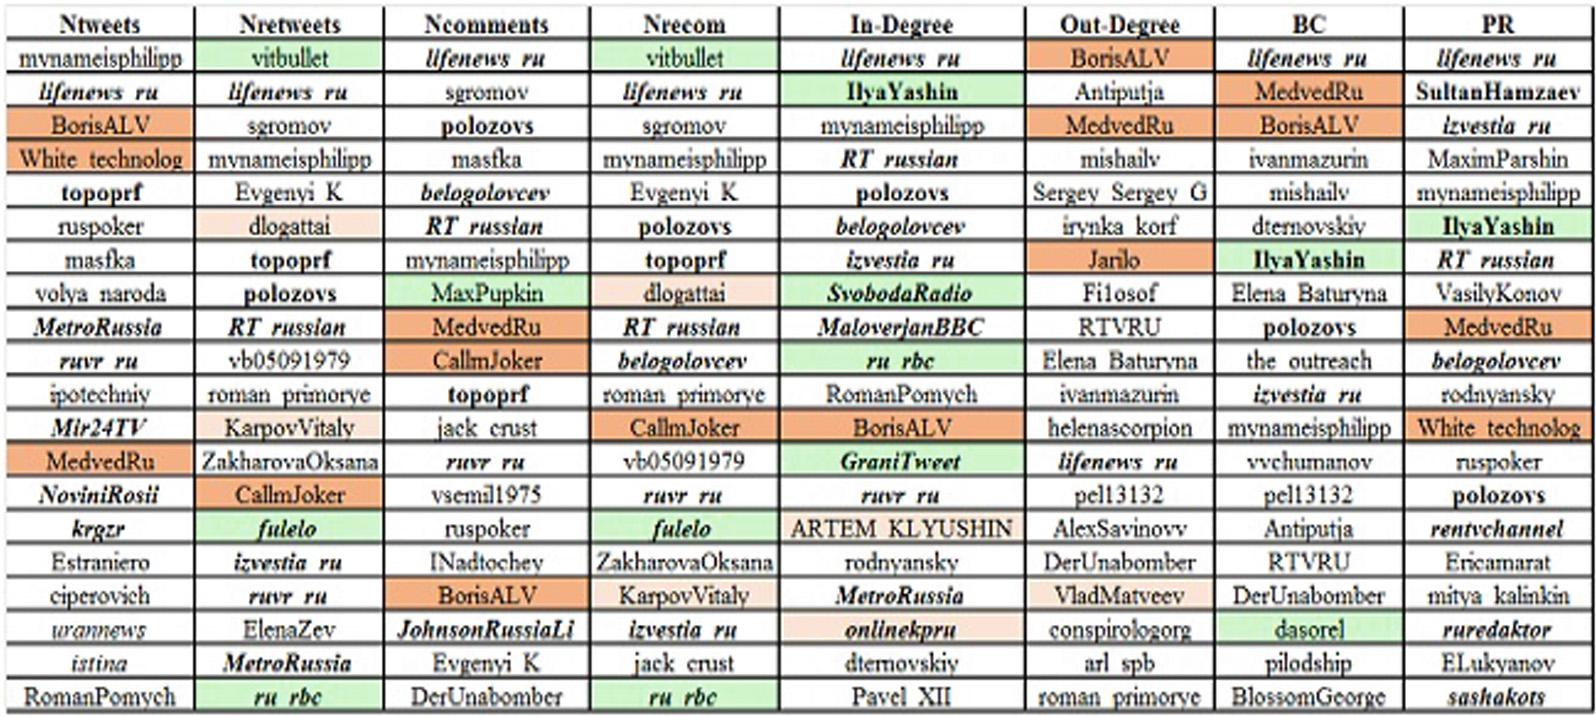
\includegraphics[scale=1.0]{topUsersRussia}
	}
	\caption{Institutional belonging and pro/contra-migrant positioning of top users in Russia.}\label{fig:topUsersRussia}
\end{figure} 

\begin{figure}[ht]
	\centerfloat{
		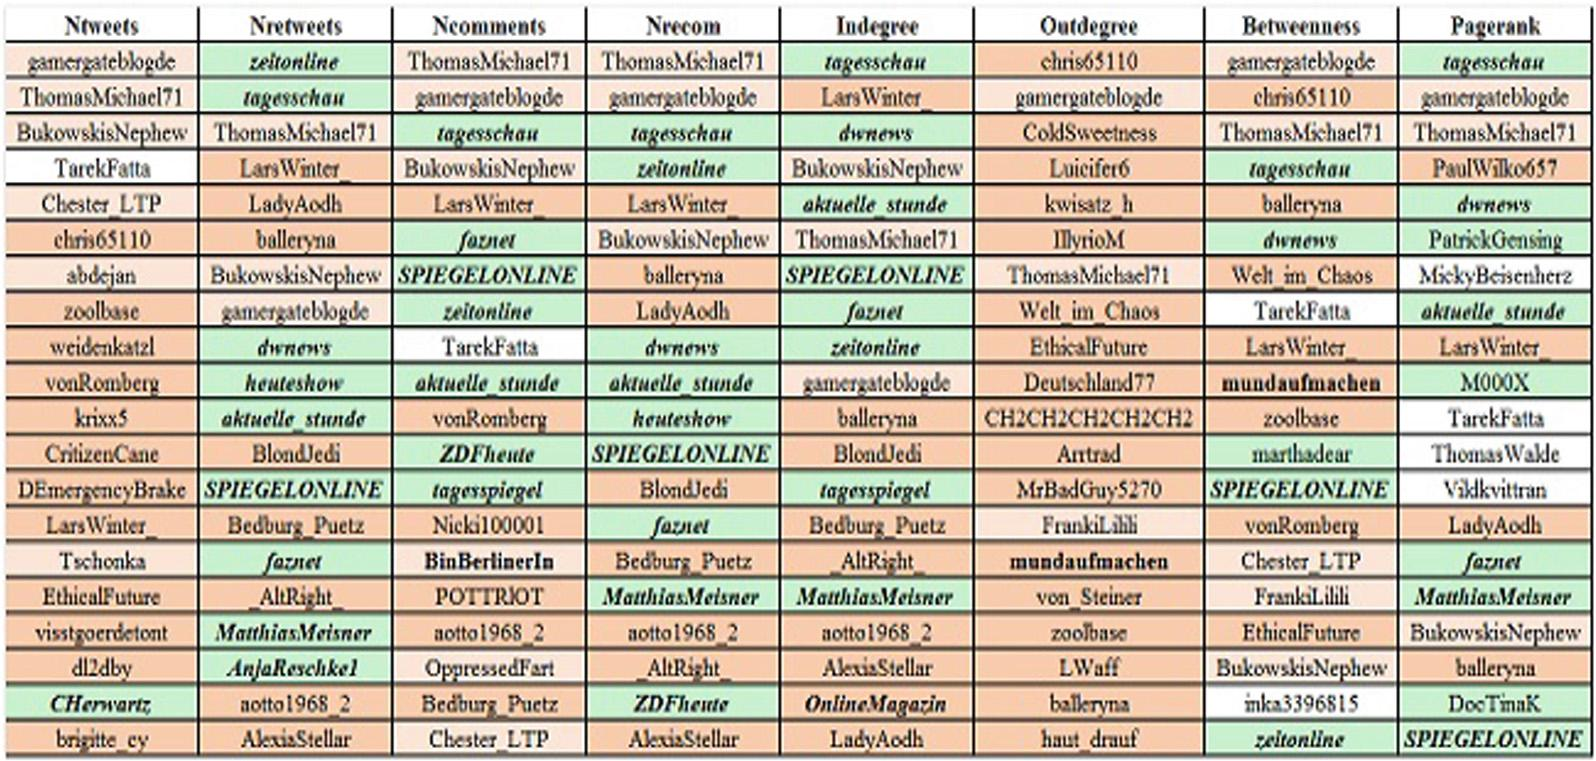
\includegraphics[scale=1.0]{topUsersGermany}
	}
	\legend{
		Regular -- ‘ordinary user’ \\
		Bold -- institutional user/representative \\
		Bold italic -- media account/journalist \\
		Italic -- ‘Twitter media’ \\
		Green -- strong/institutional support of migrants (absent from picture)\\
		Light green -- weak support of migrants \\
		White -- neutral user \\
		Light orange -- weak anti-migrant attitude \\
		Orange -- strong anti-migrant attitude/nationalist account.
	}
	\caption{Institutional belonging and pro/contra-migrant positioning of top users in Germany.}\label{fig:topUsersGermany}
\end{figure} 

\subsubsection{5. Results}

\paragraph{RQ1. Number of Tweets and Discussion Centers.} For both countries, the more users post, the more likely they become both ‘marketing’ (by \(N_{retweets}\) and \(N_{comments}\)) and ‘deliberative’ (by betweenness and pagerank) influencers, despite the difference in the size of datasets. The correlations remain in place for all the metrics for full and active-user datasets, despite the fact that elimination of ‘the crowd’ significantly drops outdegree for the Russian discussion and high values for \(N_{comments}\) and betweenness centrality for Germany. All in all, strength of the correlations remains comparable for all four of our datasets (though higher for Germany for the two aforementioned metrics), which might be telling of the nature of \textit{ad hoc} discussions on Twitter, but can also support the idea of the mediating role of \(N_{tweets}\); this needs further exploration.

But if we look closer at correlation values, we will see that outdegree correlates more weakly with \(N_{tweets}\) than other metrics throughout our data; this might mean that tweeting a lot does not provide for necessarily becoming commented or retweeted; the value is never higher than 0,418, and thus, the correlation is weak enough. Also, only in the German case, \(N_{retweets}\) matters for getting higher betweenness and pagerank, while in Russia their correlation is much weaker. But what, instead, seems to be important for becoming an influencer is a user’s indegree, that is -- how many users have interacted with you. This parameter becomes more important for becoming an authoritative node than the number of tweets, retweets, or comments -- the metrics that many works stated as markers of influencers. For all four of our datasets, the strength of ties between indegree and pagerank is 0,804 or higher. That is, a successful strategy within an \textit{ad hoc} discussion might be not to comment many times or get into a long meaningful discussion but to make a bigger number of users comment on you, perhaps by commenting them as well. On the other hand, outdegree does not seem to matter much for both betweenness and pagerank; this brings us to the conclusion that attractive content (which makes users interact with it) may be more important within such discussions than user activity.

\paragraph{RQ2. Institutionalization of the Discussion.} In Figs.~\cref{fig:topUsersRussia} and~\cref{fig:topUsersGermany}, we have marked institutional users, including media, bold (media -- bold italic). In general, the picture is similar in both countries and may be described as ‘liberal media against individual nationalists’. What is similar (and striking) in both countries is the absence of the much-awaited national/regional authorities, as well as NGOs and human rights watchers. We cannot prove dominance of institutional accounts over ‘ordinary users’, unlike in previous research \cite{XuSangBlasiola}, as we find only two politicians and one account of Public Advisory Chamber among the Russian top users, and two NGO-like organizations in the German top user lists.

Also, we cannot prove absence of nationalists as top users: in both countries, they are not only present but demonstrate blooming activity, and if in Russia they are most active in commenting, in Germany they lead both tweeting and commenting activities, all of them being non-institutionalized.

We call the picture similar, despite that, from Figs.~\cref{fig:topUsersRussia} and~\cref{fig:topUsersGermany}, the German discussion seems highly radicalized and the Russian one shows a lot of neutral users. But this may be explained by two factors. First, Biryuliovo happened over three years ago, and assessment of the accounts of top users does not bring over a lot of anti-migrant posts; this has cast its impact upon our allocation of users as neutral or biased. But we need to state that we have discovered a dominant mood among Russian ‘ordinary people’ which may be described as ‘angry patriotism’: today, such users (over a dozen in the Russian top lists) express ‘patriotic’ views like supporting Donbass population or tweeting on national pride (e.g. on leading industries like aviation, military equipment etc.) but at the same demonize the current country’s leaders as corrupt and ineffective. Thus, these users are highly politicized, no less than the German users; it is just not always possible to deduce their attitude from the tweets of the discussion (especially if they retweeted other accounts) and today’s tweets. Second, some media accounts in the Russian list (like lifenews\_ru, izvestia\_ru, or RT\_russian) were marked neutral, as we could not find direct proof of their anti-migrant bias, but their overall tone is pro-establishment, and thus their position fluctuates from supporting the state views on open visa regime for Central Asian post-Soviet ethnicities to populism of attaching social and cultural threats to their communities. Having said this, we can consider the situation similar indeed in both cases, as it is highly polarized, full of political criticism, and intolerant.

\paragraph{RQ3. The Place of Media in the Discussions.} Media, indeed, occupy a significant place in the discussion and represent a variety of political views and positions. Unlike on Russian Facebook, in this discussion both pro-establishment and highly oppositional media (ru\_rbc, GraniTweet), as well as foreign liberal media and journalists (MaloverjanBBC, fulelo, SvobodaRadio) are present, and the liberal-oppositional media show their efficacy, as they become retweeted and commented by many people without tweeting a lot. In Germany, it is mainstream media, and mostly newspapers, that also become influencers without posting a lot; they get retweeted and commented in general and by a lot of users in particular, and gain high pageranks. But even if so, media do not outperform nationalist users, and they do not get high betweenness centrality, which means that they do not play the role of ‘information mini-hubs’ as the basic nodes of the online public sphere. They remain authoritative (especially in Germany), but the niche of ‘deliberative connectors’ remains free and is occupied by the most polarized users. Thus, the ‘opinion crossroads’ may be there in terms of representation of views within the whole discussion but it is still a question whether the opposing views actually have a chance to meet.

\paragraph{RQ4. Neutrality of Top Users.} As already stated above, neutrality of users cannot be proven, especially in case of Germany. In Russia, general negative politicization of the audience goes along with nationalist and pro-nationalist views, and in Germany the discussion after a major public harassment is shaped not by the forces countering intolerance but by openly anti-migrant discussants; in both cases, it is individuals that polarize the discourse against re-settlers and media that counter this -- even if due to different reasons. Thus, for most of the German media, supporting immigrants is a non-valent issue, and expressing an alternative position would amount to a scandal. In Russia, the division between pro-establishment and oppositional media is also true for the migration issues, and thus liberal-oppositional media support their political standing by expressing pro-migrant views.

\subsubsection{6. Conclusion}

We have looked at two \textit{ad hoc} discussions on violent inter-ethnic conflicts, namely the Biryuliovo bashings in 2013 and mass harassment in Cologne in 2016, to see whether in such discussions user activity leads to higher positions within the discussion network and higher connectivity. Along with this, we assessed the substantial features of top users, such as their institutional status and opinion positioning.

Despite the differences in samples, we have managed to show that comparing influencers is possible, and there are patterns in the structure of influencing that are similar. The main methodological finding is that, in both discussions, the number of users involved mattered more for becoming an influencer (by BC and PRC) than the number of actual tweets, retweets, or comments received by a user.

Though direct comparisons were not always possible by our methodology, we have found more similarities in the two cases than we had expected. Thus, in both countries, the situation may be described as opposition ‘liberal media vs. nationalist users’, and the absence of both authorities and NGOs is striking. Media do become influencers, but in terms of authority (or ‘marketing’ approach) rather than in deliberative terms, as they do not get high betweenness centrality and thus may have difficulties in performing the roles of shapers of information flows. In both countries, the discussion was highly opinionated and emotionally heated even within several weeks after the events, and seemingly higher neutrality of the Russian users was compensated by their overall politicization and rebuttal modus.

Thus, as to the question of whether and how ‘opinion crossroads’ are forming, there is evidence that, in general, left-right or in-system/oppositional views are well represented by media within the discussions. But virtual absence of pro-migrant institutions and opposition of liberal media to pro-nationalist ‘ordinary users’ shows that, in both countries, the discussion is far from being balanced, rational, and inclusive.

\section{Анализ пользовательских дискуссий}\label{sec:ch2/sec5}

\subsection{Content Sharing in Conflictual \textit{Ad-Hoc} Twitter Discussions: National Patterns or Universal Trends?}\label{subsec:ch2/sec5/sub2}

\subsubsection{1. Introduction}

In the last decade, online content selection and news spreading proved to be ‘a phenomenon of growing social, economic and political importance’ \cite[p.~331]{LeeMa} capable, arguably, of subversion of traditional media gatekeeping \cite{Carr}. In 2010s, research on factors influencing content sharing has dealt with user motivations and content exposure concepts, among which selective exposure theory shows significant explanatory power; but, till today, these studies provide mixed evidence on which particular factors influence more the selection of shared content, and they remain case-oriented and lack comparative perspectives.

In neighboring research zones, content selection has been studied for decades; thus, of media effects studies, gatekeeping theory is the closest to the studies of content sharing, as it has for long been based on similar sets of research questions. Today, this theory expands to a much greater variety of gatekeeper types, and multi-layer (primary vs. secondary, as well as other divisions) gatekeeping is discussed. But these studies suffer from the same shortcomings; also, the studies do not involve the context of media systems as a variable, while it inevitably casts impact upon the spectra of available content.

This paper aims to partially cover these gaps by analyzing secondary gatekeeping patterns within three Twitter discussions on recent ethnic/racial conflicts in the USA, Russia, and Germany. Here, comparability comes from their \textit{ad hoc} nature \cite{BrunsBurgess} as well as from similarity of the cases in terms of political polarization and policy implications.

Using a specially developed web crawler, we collected the bulk of the discussions, ranged the users by the number of tweets, and assessed the links to outer content in 1,000+ tweets by active users for each case by six variables. In Sect. 1, we present the overview of the research approaches, including primary vs. secondary gatekeeping. In Sect. 2, the cases and the hypotheses are presented. In Sect. 3, we describe data collection, sampling, and coding. In Sect. 4, we provide the results and test the hypotheses. In Sect. 5, we discuss our contribution to the existing research and the limitations of the study.

\subsubsection{2. Explaining Patterns of Content Sharing: Research Approaches}

Today, content sharing encompasses sharing the same content within a platform (e.g. retweeting) and selection and re-publication of media content from outside the platform -- or both, with no distinction in many of published works. Since early 2000s, the researchers have tried to conceptualize and empirically assess the motivations and patterns of content sharing on social media platforms. One of the approaches was uses and gratifications theory which focused on user motives for sharing, finding out that these were, primarily, information seeking, socializing, entertainment, and status seeking  \cite{LeeMa}, especially on online networks as content sharing communities \cite{LeeAntoniadisSalamatian}. Later, network-based approaches added to this evidence that weakly tied users were more likely to share content if they are tied uni-directedly, rather than bi-directedly, thus forming an evidence of content sharing hierarchies in social media \cite{ShiRuiWhinston}

Another research stream tries to identify the factors that influence content selection beyond user motivation. Recently, a range of works tried to check whether the selective exposure theory \cite{SearsPreedman} works for social media -- that is, whether information shared by the users is in line with their values, beliefs, and biases. So far, there is mixed evidence whether this theory works well for content sharing, e.g. on Twitter. For example, authors \cite{ThorsonWells} have shown that, during London riots of 2011, users shared tweets that were in line with their beliefs; in experiment-based research, users do tend to demonstrate bias in news selection \cite{MunsonResnick} -- to the extent of formation of echo chambers \cite{Garett} with the same views reproduced. A group of Italian and American researchers have demonstrated that the selective exposure theory, especially when it comes to personal traits and beliefs, can explain the polarizing effects in echo chambering \cite{QuattrociocchiCaldarelliScala}, consumption of (fake) news \cite{BessiCaldarelliDelVicario}, and in formation of scientific networks \cite{QuattrociocchiAmblardGaleota}. Most echo chambers research is, though, focused on studying in-platform content exchange and its effects (for a review, see \cite{Bessi}), including spreading of online behavior \cite{Centola} and raising issues via collective intelligence \cite{Levy,MaloneKlein}. On the other hand, authors \cite{MorganLampeShafiq} have proved that in sharing news from outside Twitter, users tend to include into their shared links media of various political stands; similar findings were reported for Youtube \cite{HalveyKeane}.

But in both cases, the role of content attracted from outside the platform in formation of user echo chambers remains understudied; we still do not know how this or that piece of content is selected and what makes it attractive enough to break the cross-platform boundaries. Also, being well-grounded in theory, this research remains case-oriented and often lacks comparative component; we try to partly cover this gap.

\paragraph{Content Selection and Gatekeeping.} Mechanisms of content selection for (re)publication were traditionally studied in media effects research, and in particular -- in studies of gatekeeping \cite{White1950}. In general, gatekeeping helps reduce the complexity of the world turning the incoming unstructured information flow into limited and structured sets of comprehensible messages \cite{Singer}. Also, as early as in 1975 \cite{Janowitz}, gatekeeping was associated with objectivity model of journalism based on impartiality and balance, as opposed to advocacy model. But from the very early days of gatekeeping research, it was also considered an oppressive mechanism allowing non-professional intentions in news selection \cite{Mills}.

Media have for decades been studied as major societal information gatekeepers. In 1980s to 1990s, the gatekeeping theory focused on structural constraints of information selection \cite{DonahueOlienTichenor}, of which time and space pressures, professional values, and organizational routines seemed to be more important than the type of platform, thus forming cross-media understanding of news selection priorities. Also, for international gatekeeping, news values theory was used to explain the choice of local/national vs. international news \cite{RobertsBantimaroudis}.

The growth of Internet has drastically changed the gatekeeping landscape. Media institutions felt they were losing monopoly in gatekeeping -- that is, the control over the relationship with the users they had previously prospered with. Industry predictions ranged from alarmist claims of the ‘collapse of gatekeeping’ \cite{WilliamsDeliCarpini} to transformationalism. Among the latter, several ideas deserve mentioning. Thus, the ‘gatewatching’ concept was suggested \cite{Bruns} assigning the users a capacity to transmit information from media without actual participation in content production. Other concepts were ‘network gatekeeping’ \cite{BarzilaiNahon} and ‘audience gatekeeping’ \cite{ShoemakerVos} that described the growing role of information consumers in dissemination of news; soon, these ideas expanded beyond the industry-based structural understanding of ‘gatekeeping layers’, and \textit{secondary gatekeeping} started to be discussed in media studies \cite[p.~6]{ShoemakerVos} \cite{RobertsBantimaroudis,White1950}. Also, today, the gatekeeping theory meets social network analysis where key nodes (users) who either disseminate information themselves or link discussion zones are considered new gatekeepers \cite{JurgensJungherrSchoen} or, rather, gatekeepers with smaller gateways \cite{BastosRaimundoTravitzki}.

Today, three gatekeeping models are most elaborated (for an overview, see [19]). For the first one, authors define five levels of analysis: individual, that of communication routines, organizational, social-institutional, and social-systemic \cite{ShoemakerVos}. For the second \cite{Nielsen}, primary gatekeepers are those ‘who by filtering information and publishing decide what is specifically what we commonly understand as news’; secondary gatekeepers ‘are those that filter already available news content’. Thus, it directly links primary gatekeeping to editorial work, and secondary gatekeeping to content sharing (link-, affinity-, or community-based). The third one \cite{ThorsonWells,WellsThroson} shifts from selection to ‘curation’ of content and suggest five types of curators: journalists, strategic communicators, ‘social others’, computer algorithms, and a reader’s self \cite[p.~35]{WellsThroson}
.
We, though, need to state that we see the distribution of primary/secondary gatekeeping role to be much more complicated than it comes from the current academic debate, and a ‘two-step gatekeeping process’ \cite{Singer} reflecting the idea of two-step communication flow \cite{Katz}, is just one of options. To reduce the complexity, we define them as content producer (‘primary gatekeeper’), content re-publisher (‘secondary gatekeeper’), and intermediary (‘tertiary gatekeeper’). Primary gatekeepers are those who produce pieces of content originally; the content may as well be user-generated. In contrast to this, secondary gatekeepers, when re-publishing, are considering what might be interesting for their core information cocoon. This division seems to be a key one, as their final goals may be similar, as well as factors that shape the individual level of decision-making (from ideology to personality \cite{ShoemakerReese}), ‘resulting in choices that are organizationally efficient and culturally acceptable inside and outside the newsroom’ \cite[p.~56]{Singer}. Tertiary, or ‘algorithmic’ \cite{Napoli} gatekeepers, in their turn, use storage, aggregation, and affinity-based algorithms to shape the overall picture.

What differentiates ‘new’ and ‘old’ gatekeepers is selection principles as part of the ‘content curation’ process. For all of them, the issue of subjectivity in selection has never been resolved: in the 50s and 60s, while it was argued that editors were stuck into the machinery of editorial choice based on vigorous criteria \cite{Gieber}, other authors \cite{Snider,White1950} argued that subjectivity was the basic principle for content selection. With mediatization of society \cite{EsserStromback,Hjarvard}, this gap in understanding has only deepened, as media logic itself has become more subjected to various social pressures, some seen as external for editorial offices and some explicating in subjective editorial decisions. But in online user-level content sharing, user decisions become even more individualized and hectic, also due to combining random/purposeful decisions based on personal traits \cite{Bessi} with the impact of tertiary gatekeepers.

\subsubsection{3. Twitter Discussions as Research Object: The Three Cases}

Of all social media, Twitter has been under researchers’ particular scrutiny due to its bigger feasibility, availability of research software, and platform features. Several works \cite{BakshyRosennMarlow,ShiRuiWhinston} have stated that Twitter is for content dissemination more than other social networks are. Here, we need to discuss how peculiarities of Twitter discussions \cite{ChaBenevenutoHaddadi} and relations between Twitter and the outer media system affect content sharing.

First, we need to acknowledge that replicability of our findings to other discussions may be low due to the \textit{ad hoc} nature of the event-based discussions \cite{BrunsBurgess}. This may lower the comparative potential and be viewed as a natural limitation of this research, even if we have no empirical proof of non-replicability.

Second, the network structure of the discussion, including echo chambers and influencers \cite{BodrunovaBlekanovMaksimov}, may also play a role in content selection -- or, rather, content selection helps shape echo chambers, as it is natural to suggest that the logic of consonant reality \cite{NoelleNeumann} is shows up in all user decisions, including content sharing. In our previous \cite{BodrunovaLitvinenkoGavraYakunin,BodrunovaLitvinenkoBlekanov2016} and ongoing research on Germany and Russia, we have noticed that echo chambers are not only based on attitudes towards immigrants but also on user type. Thus, in Germany in 2014 and 2016, pro-migrant camp is formed around left-liberal media and NGOs, while the pro-nationalist one -- around nationalist leaders in Germany and Switzerland who look like ‘ordinary users’. In the Russian case, under the cover of intense tweeting by media, we discovered a chain of similar pro-nationalist ‘ordinary users’ who also acted as gateways for each other’s content. We may, thus, hypothesize that cross-platform content sharing is linked to the user type, as well as to his/her attitude towards the minority under question.

Third, what may also matter is the difference of media systems and the role of Twitter in them. Russia differs from both Germany and the US in terms of low trust to print media, competitive social media market, and low hybridization of TV. The US and Russian media markets have a distinct online-only segment, while in Germany dominant positions on offline market survive online. All the media systems have relatively high media-political parallelism, and one can trace political alienations in media content and endorsement: progressive/conservative in the US, left/right in Germany, and pro-/anti-systemic in Russia \cite{BodrunovaLitvinenko2013,BodrunovaLitvinenkoGavraYakunin}. As to the Twitter’s position on the media markets, its market niche is a bit bigger in the US than in Germany and Russia; there is lack of substantial research on the comparable user profiling in the three countries.

Thus, we formulate the following RQs: (1) is the pattern of content sharing national-bound or universal? Do established media remain the leading primary gatekeeper for Twitter users in \textit{ad hoc} discussions? Do we see any differentiating impact of the outer media systems upon content sharing? (2) Does the type of secondary gatekeeper correlate with the type of primary gatekeeper? (3) Do personal biases of the secondary gatekeeping correlate with the type of the primary gatekeeper and the views in the attracted content?

\paragraph{The Cases Under Scrutiny.} To better formulate our hypotheses, we will also shortly describe the cases we look at.

In Russia, in October 2013, a Muscovite Egor Scherbakov was, allegedly, killed by an Uzbek immigrant Orkhan Zeynalov; later, Zeynalov was arrested and found guilty. Before the trial, local residents committed repeated bashings of a major warehouse in the Moscow district of Biryulyovo where the migrant community dwelled and worked; they raised against police and formed ‘people’s brigades’ to monitor the local area. The case became the most resonant conflict between Russians and Southern re-settlers in the recent Russian history.

In the USA, in August 2014, a white police officer Darren Wilson shot dead an unarmed African American youngster Michael Brown. Peaceful protest and violent riots rose repeatedly in Ferguson, Missouri, as well as all over the US. The case has polarized American society not only along white/non-white lines but also across political affiliations. 

In Germany, in the New Year night of 2016, mass sexual harassment of women by alleged migrants from Middle East and North Africa took place in Cologne. This made people in many cities protest, mostly under the PEGIDA movement slogans. National media were practically silent on the case, as editorial guidelines prevent journalists from covering ethnics origin of the criminals, while local media reported the case.

\paragraph{Research Hypotheses.} Having stated all the mentioned above, we have formulated the following hypotheses:
\begin{itemize}
	\item H1. Across the cases, an ‘onion’ pattern of content sharing will emerge: social media will be shared most; online-only media will follow, traditional media will come third. In general, structures of media systems will have no visible impact upon content sharing patterns.
	\item H2. The type of secondary gatekeeper will correspond with that of primary gatekeeper in all the three cases.
	\item H3. Personal preferences (pro-/anti-minority) of users will correlate with the type of primary gatekeeper, as well as with pro-/anti-minority bias in shared content.
\end{itemize}

\subsubsection{4. Methodology}

To test the hypotheses, we have collected the discussion content, formed tweets datasets for manual coding, coded them, and made calculations for H1 and descriptive statistics (Cramer’s V) for H2 and H3.

\paragraph{Data Collection.} We have used vocabulary-based web crawling for data collection. To form the vocabularies, we have collected and manually assessed relevant keywords and hashtags at trendinalia.com; all the cases were in Twitter trending topics for at least two days. We have also added keywords found via manual snowballing in 1,000+ popular tweets per case. We used the crawler developed earlier with modules modified for our purposes. The uploading periods included October 1 to 31, 2013 for Russia, August 22 to 31, 2014 for the USA (as the peaking dates of the conflict, August 14 to 21, contained an unfeasible number of tweets for our software), and January 1 to 30, 2016 for Germany. The uploads returned 10715 tweets by 3574 users for Russia, 193812 tweets by 70018 users for the US, and 64874 tweets by 12382 users for Germany.

\paragraph{Sampling of Datasets for Data Annotation.} As we were interested in the active users’ content sharing patterns, we have formed feasible datasets of tweets for assessment based on user lists ranged by quantity of the published tweets. The collections had to be feasible for manual coding, and thus we were seeking the datasets containing around 1000 tweets; for further research, the datasets are to be enlarged. We had to cut the long tail of the discussion, which may have affected the results in terms of the variety of content shared; but the reason for looking at most active users was that they tend to have more stable patterns of posting and content sharing. Thus, our sample is not representative, but randomized sampling would have even distorted the results in a way, as active users are also those who are retweeted more than others \cite{BodrunovaBlekanovMaksimov}, and, thus, the content they share creates impact that goes beyond average.

Cutting the user ‘long tail’ implied establishing a threshold of user activity -- that is, the minimum number of tweets posted in the discussion \cite{Chadwick,MunsonResnick}. Due to very differing user activity, these thresholds (\textit{K} = \textit{Ntweets} per user) differed much: for Russia, \(K = 20\), for the USA, \(K = 66\); for Germany, \(K = 10\); \(K\) was defined as the point where the graph that ranged users stopped to drop significantly from user to user. After that, randomized samples (certain percentage of tweets) from each user were taken depending on the overall user activity in the discussion, to preserve the comparable volume of the datasets: for Russia, 40\%, for the USA, 5\%, for Germany, 30\%. After cutting out irrelevant tweets, replicas, and foreign-language tweets, the final datasets included: for Russia, 1120 tweets; for the USA, 1095 tweets; for Germany, 911 tweets (since many tweets were in English and had to be cut out). The relatively small sample is explained by the fact that reading of media texts could not be automatized, as so far no sentiment analysis or machine-learning techniques could provide for clear understanding of user attitudes.

\paragraph{Coding.} 
Coding. Coding of the datasets was performed by experienced experts and native speakers. Four variables were coded: user type = secondary gatekeeper type (‘ordinary user’/political activist/political actor/hybrid media/online-only media/‘media’ on Twitter/‘culture’/other or non-defined); user’s attitude to minority (neutral/pro/anti/non-defined); type of primary gatekeeper (‘social’, online-only, hybrid media, politics, ‘culture’, other/non-defined); attitude to minority in media content (neutral/pro/anti/non-defined). Links to own content were excluded from the analysis. Also, we excluded the links to Twitter-based photo content (pic.twitter.com). In future, bigger samples may be coded.

\subsubsection{5. Results and Discussion}

On completing the aforementioned procedures, we have received the following results.

\textit{H1.} We have calculated the number of links to content outside Twitter in the three
datasets in absolute figures and in \% (see Table~\cref{tab:datasetLinkNumber}).

\begin{table}[ht]%
	\centering
	\caption{Number of links in the datasets, absolute \(N\).}%
	\label{tab:datasetLinkNumber}% label всегда желательно идти после caption
	\begin{adjustbox}{width=1\textwidth}
		\small
		\begin{tabular}{ c  c  c  c  c  c  c  c  c  c  c }% Вертикальные полосы не используются принципиально, как и лишние горизонтальные (допускается по ГОСТ 2.105 пункт 4.4.5) % @{} позволяет прижиматься к краям
			\toprule
			Country & \multicolumn{2}{l}{\makecell{All links, of all tweets}} & \multicolumn{2}{l}{\makecell{Social media}} & \multicolumn{2}{l}{\makecell{Online-only media}} & \multicolumn{2}{l}{\makecell{Hybrid media}} & \multicolumn{2}{l}{\makecell{Other}} \\
			\hline
			Russia & 159 & \textit{14.2\%} & 62 & \textit{39\%} & 29 & \textit{18.2\%} & 62 & \textit{39\%} & 6 & \textit{3.8\% } \\
			USA & 280 & \textit{25.5\%} & 70 & \textit{25\%} & 96 & \textit{34.3\%} & 67 & \textit{23.9\%} & 46 & \textit{16.4\%}       \\
			Germany & 317 & \textit{34.8\%} & 41 & \textit{12.9\%} & 41 & \textit{12.9\%} & 197 & \textit{62.1\%} & 38 & \textit{12\%} \\
			\bottomrule
		\end{tabular}%
	\end{adjustbox}
\end{table}

In Table~\cref{tab:datasetLinkNumber}, we show political, economic, and cultural links all together, as they are few; everywhere, media are, indeed, the dominant primary gatekeeper, but with very different roles of various types of media. This is why we describe the cases in more detail here.

In the Russian case, we see a picture of rivalry between social and hybrid media -- despite low structural online/offline parallelism and low trust to legacy media in Russia. Thus, the idea of the ‘onion’ pattern of content sharing is not supported; hybrid media are shared more than expected. Social media are represented by blog platforms (Livejournal, Blogspot), the local social network Vkontakte and global Facebook and Instagram, and video hostings (Youtube, Ustream). More interestingly, if we look at online-only and hybrid media in terms of their political bias (and to several political links), we will see that, on Russian Twitter, pro-elite and liberal-oppositional content is shared almost equally, making Twitter much closer an ‘opinion crossroads’ than, e.g., the Russian Facebook, a distinct platform-wide echo chamber, as stated earlier \cite{BodrunovaLitvinenkoGavraYakunin}.

For the American case, we see a picture opposite to the Russian one. Here, only 25\% of the links is to social media and other 24\% -- to hybrid media, while online-only comprise over one third. For America, the ‘onion’ pattern, again, is irrelevant. Also, there are several other features characteristic for the US case. First, all the variety of the mainstream media is shared. The leading print media included \textit{Los Angeles Times}, \textit{The Nation}, \textit{The Atlantic}, \textit{Chicago Tribune}, \textit{USA Today}, \textit{Time}, \textit{The Washington Post}, and \textit{The New Yorker}; of TV, MSNBC, CBS, CNN, and Fox got 2 to 3 links each. Regional media market is well-represented, especially by media of the St.Louis county. Second, there is a striking diversity in formats and political positions of online-only media, many of them being personal or group providers of opinionated writing, grassroots political reporting, and alternative news (like \textit{RawStory.com}, \textit{Madiaite.com}, \textit{Vox}, or \textit{Breitbart}). Some outlets balance between politics and journalism (\textit{TheConservativeFreeHouse}, \textit{ThinkProgress}, \textit{TalkingPointsMemo}, \textit{AmericanThinker}). This diversity is supported by that in political links (8\% of all links) belonging to activist, human-rights, and petition websites. Third, we have found virtually no African American media. Unlike in the tweets, the ‘attracted’ discourse, be it pro- or anti-Black, seems to be shaped by ‘white’ media -- except for Youtube that features eyewitnesses’ views, African American commentators, and rap music in support of Mike Brown.

The German case is the only that proves H1 right, but, again, the ‘onion’ logic does not fully work, as social and online media get equal quantity of links -- both almost five times less than the hybrid media. 26 links, or 8,2\%, belong to political organizations or activists. Surprisingly, 84 of 186 (45\%) of German hybrid media links are to advocacy outlets, but this may be explained by the fact that 70\% of them lead to a right-wing magazine \textit{Zuerst} and are posted by the same user. Of the rest, 46 are supra-regional general-interest and 50 are regional and local general-interest media. The regional distribution is representative enough; the links are not Cologne-centered. Nearly all the big players are also present: newspapers (\textit{FAZ}, \textit{Süddeutsche Zeitung}, and \textit{Die Welt} to \textit{Handelsblatt} and the tabloid \textit{Bild}), news magazines (\textit{Spiegel}, \textit{Focus}), public and commercial TV, and public radio. Due to this, left-right media market polarization reconstructs in the discussion, with right-wing media clearly winning. Online-only media referenced to are also highly politicized. More than half of them (24 out of 41) are the links to advocacy media fostering agendas and news frames alternative to the mainstream media, like \textit{Alternative Dresden News}, \textit{DortmundEcho}, or \textit{Pi-news}.

Thus, our H1 is fully rejected: the ‘onion’ pattern of content sharing is absent. Also, national media systems and the state of civil society seem to have a bigger impact than expected upon the sharing strategies of the users. While in the US and Germany 9\% and 8\% of the links, respectively, belong to political websites, Russian content sharing is depoliticized. What unites all the cases, though, is an ‘opinion crossroads’ in terms of political bias present via media links platform-wide, but it is yet unclear whether it is present within ‘echo chambers’.

\textit{H2 and H3.} To assess correlations between secondary gatekeepers’ types and attitudes to minorities vs. primary gatekeepers’ types and attitudes in their content, we have conducted Cramer’s V for the 4 variables described above. The results are shown in Tables~\cref{tab:gatekeeperTypeVS} and~\cref{tab:gatekeeperAttitideVS}.

\begin{table}[ht]%
	\centering
	\caption{Number of links in the datasets, absolute \(N\).}%
	\label{tab:gatekeeperTypeVS}% label всегда желательно идти после caption
	\begin{adjustbox}{width=1\textwidth}
		\small
		\begin{tabular}{ c  c  c }% Вертикальные полосы не используются принципиально, как и лишние горизонтальные (допускается по ГОСТ 2.105 пункт 4.4.5) % @{} позволяет прижиматься к краям
			\toprule
			& $\ldots$primary gatekeeper type & $\ldots$attitude to minority in primary gatekeeper’s text \\
			\hline
			Russia & 0.220 & \textbf{0.248*} \\
			USA & \textbf{0.183**} & \textbf{0.208**} \\
			Germany &\textbf{ 0.219*** } & \textbf{0.372***} \\
			\bottomrule
			\multicolumn{3}{@{}p{\textwidth}}{%
%				\vspace*{-4ex}% этим подтягиваем повыше
				\hspace*{2.5em}% абзацный отступ - требование ГОСТ 2.105
				Sig.: \(*p \le 0.05\); \(**0.05 < p \le 0.001\); \(***p < 0.001\).
			}\\
		\end{tabular}%
	\end{adjustbox}
\end{table}

\begin{table}[ht]%
	\centering
	\caption{Number of links in the datasets, absolute \(N\).}%
	\label{tab:gatekeeperAttitideVS}% label всегда желательно идти после caption
	\begin{adjustbox}{width=1\textwidth}
		\small
		\begin{tabular}{ c  c  c }% Вертикальные полосы не используются принципиально, как и лишние горизонтальные (допускается по ГОСТ 2.105 пункт 4.4.5) % @{} позволяет прижиматься к краям
			\toprule
			& $\ldots$primary gatekeeper type & $\ldots$attitude to minority in primary gatekeeper’s text \\
			\hline
			Russia & \textbf{0.288***} & \textbf{0.290***} \\
			USA & 0.150 & \textbf{0.350***}  \\
			Germany & \textbf{0.183***} & \textbf{0.401***} \\
			\bottomrule
			\multicolumn{3}{@{}p{\textwidth}}{%
%				\vspace*{-4ex}% этим подтягиваем повыше
				\hspace*{2.5em}% абзацный отступ - требование ГОСТ 2.105
				Sig.: \(*p \le 0.05\); \(**0.05 < p \le 0.001\); \(***p < 0.001\).
			}\\
		\end{tabular}%
	\end{adjustbox}
\end{table}

As we see from Tables~\cref{tab:gatekeeperTypeVS} and~\cref{tab:gatekeeperAttitideVS}, in all the cases, type and attitude of the secondary gatekeeper (that is, Twitter user) weakly but significantly correlates with bias in the shared text -- that is, the hypothesis of selective choice of content is supported in cross-country perspective, and in Germany these ties are the strongest. But at the same time the type of primary gatekeeper (that is, in most cases, media platform) has varying relevance. Thus, in Russia, users of various nature all rely on a variety of media, from hybrid to social, but still choose the content that supports their views; this means they look more at content than stick to their preferred media outlets. In the US, the position of a user towards the minority does not correlate with where a user goes for his/her information supply; it is the particular attitude that will be sought after, and this also may be a sign of occasion-based content consumption and sharing, as there is no stability in linking to the same source. That is, echo chambers in content sharing seem to exist in all the cases, but they are formed via different mechanisms. The type of links seems to be all in all less important for the users than the content, and this supports the idea of active seeking of information rather than ‘information cocooning’ and passivity in content consumption. But, as already stated, this may also support the idea of occasional sharing as soon as the users run into the content that supports their views. This needs further research.

What is also seen is that our idea of collision of the individual and organizational levels of gatekeeping may be supported in future. What we have definitely seen in case of Germany and for several users in the US and Russian datasets is what one may call ‘individual-level filter bubbles’ formed not only via posting but also via content sharing. This may amplify the echo chamber concept, as not only network-level inter-user information exchange but also individual-level filtering leads to the rise of closed-up communicative zones. In our future work, we will try to see in detail which gatekeepers were on which side of the conflict, with bigger samples allowing for better conduct of regression analysis.

\paragraph{Discussion and Limitations.} Several methodological issues rose in the process of dataset formation and coding. Thus, representativeness of the datasets was considered against feasibility, and the decision was to have more users, rather than more tweets from each user, in the datasets, especially because many most active users were posting or retweeting the same tweets multiple times and had to be almost fully eliminated from the datasets. Also, comparability of the cases and the codebooks was discussed; as stated above, the cases were considered comparable due to their political nature, time structure, and main actors involved. But still one needs to realize that the understanding of political cleavages differs much in the three countries, and in some cases bipolarism of the political spectra does not bring a proper solution in judging the content.

We could not always code the ethnic belonging of the users, and this variable was not used in the research. Manual assessment of the datasets shows much bigger presence of African American population on Twitter than migrant population in Germany or Russia (which is nearly 0), but, as we see from the results, this did not affect the results too much -- perhaps due to the structure of the media systems, since they all lack significant representation of the minorities among registered media, and this means that the users share what is available.

And, of course, it was hard not to allow a certain level of subjectivity in coding, but we hope that similarity of the codebooks, cross-checks, and advice from native speakers helped to overcome these limitations.

\subsubsection{6. Conclusion}
In this paper, we have shown that the complexity of gatekeeping in today’s commu- nication flows may be reduced to primary (content producers), secondary (content disseminators), and tertiary (‘algorithmic’) gatekeepers; thus, content sharing patterns shed light onto the relations between primary and secondary gatekeeping.

We have found that national media markets and the state of civil society still help break the cross-national patterns of content sharing on Twitter, and all the variety of views is presented. But at the same time, across cultures, users share the content they solidarize with in their views; but if in Russia and Germany, user bias is linked to the media they consume, in the USA users are more spontaneous in their choice. Thus, the idea of selective content sharing due to bias and user status is supported cross-culturally, but what is shared depends highly on what national arenas offer.

\FloatBarrier
